\documentclass{beamer}

\mode<presentation>
{
  \usetheme{Boadilla}
  \usecolortheme{beaver}
  \usefonttheme{serif}
  \setbeamertemplate{navigation symbols}{}
  \setbeamertemplate{caption}[numbered]
  \setbeamerfont{frametitle}{size=\large}
  \setbeamerfont{block title}{size=\small}
}

\usepackage[english]{babel}
\usepackage[utf8]{inputenc}
\usepackage{booktabs}
\usepackage{amsmath}
\usepackage{graphicx}
\usepackage{tikz}
\usetikzlibrary{positioning, decorations.pathreplacing, calc}
\usepackage{xcolor}
\graphicspath{{figs/}}

\definecolor{mtblue}{HTML}{1F77B4}
\definecolor{clsorange}{HTML}{FF7F0E}
\definecolor{salgreen}{HTML}{2CA02C}

\title[ViT Representation Analysis]{Representation Analysis of a Multi-Task Vision Transformer\\Probes, CKA, and Sparse Feature Decomposition}
\author[Welsh]{Nicholas Welsh}
\institute[FIT]{Florida Institute of Technology\\Department of Computer Science \& Mathematics}
\date{April 2026}

\begin{document}

\begin{frame}
  \titlepage
\end{frame}

\begin{frame}{Outline}
  \tableofcontents
\end{frame}

% ============================================================
\section{Motivation}
% ============================================================

\begin{frame}{The Question Project 2 Asks}
\textbf{Project 1's finding.} The same input produced different attribution maps depending on which of the three ViT variants was being explained.
\vfill
\begin{center}
\large \textbf{Are the three variants actually different inside, or are the explanation methods just noisy?}
\end{center}
\vfill
\small
\begin{itemize}\setlength\itemsep{2pt}
  \item Project 1's attribution methods only describe outputs.
  \item To answer the question we have to look at the activations themselves.
  \item All four main methods of Project 2 produce numbers, not heatmaps. None overlap with Project 1.
\end{itemize}
\end{frame}

\begin{frame}{Two Outcomes, Both Worth Reporting}
\small
\textbf{Outcome A: internal differences match attribution differences.} Project 1's attribution-map differences were real signal. The variants encode the input differently inside the network. Multi-task supervision genuinely changes what the backbone learns.
\vfill
\textbf{Outcome B: internal representations look the same.} Project 1's differences were noise from the explanation methods. The disagreement was an XAI-reliability story rather than a model story.
\vfill
\begin{center}
\textbf{Spoiler.} The answer is partly Outcome A. Multi-task and classifier-only are close internally. Saliency-only diverges sharply.
\end{center}
\end{frame}

% ============================================================
\section{Model and Data}
% ============================================================

\begin{frame}{Architecture: One Model, Three Loss Conditions}
\begin{center}
\resizebox{0.78\linewidth}{!}{%
  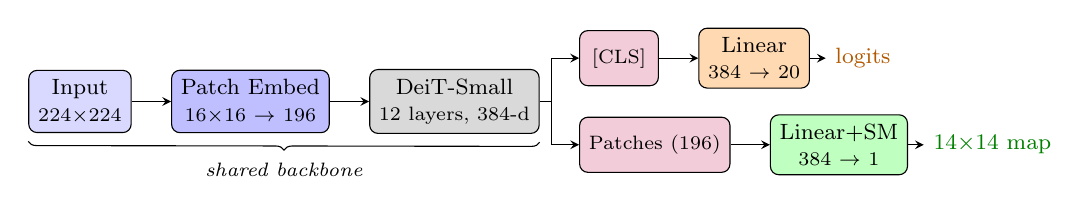
\begin{tikzpicture}[
    node distance=0.5cm,
    box/.style={draw, rounded corners=3pt, minimum height=0.7cm, align=center, font=\footnotesize},
    >=stealth
  ]
    \node[box, fill=blue!15, minimum width=1.3cm] (img)
      {Input\\\scriptsize 224$\times$224};
    \node[box, fill=blue!25, minimum width=1.4cm, right=of img] (patch)
      {Patch Embed\\\scriptsize 16$\times$16 $\to$ 196};
    \node[box, fill=gray!30, minimum width=1.7cm, right=of patch] (backbone)
      {DeiT-Small\\\scriptsize 12 layers, 384-d};
    \node[box, fill=purple!20, minimum width=1.0cm, above right=0.55cm and 0.5cm of backbone.east, anchor=west] (cls)
      {\scriptsize [CLS]};
    \node[box, fill=purple!20, minimum width=1.0cm, below right=0.55cm and 0.5cm of backbone.east, anchor=west] (ptok)
      {\scriptsize Patches (196)};
    \node[box, fill=orange!30, minimum width=1.3cm, right=of cls] (clshead)
      {Linear\\\scriptsize 384 $\to$ 20};
    \node[box, fill=green!25, minimum width=1.3cm, right=of ptok] (salhead)
      {Linear+SM\\\scriptsize 384 $\to$ 1};
    \node[right=0.2cm of clshead, font=\footnotesize, text=orange!70!black] (clsout) {logits};
    \node[right=0.2cm of salhead, font=\footnotesize, text=green!50!black] (salout) {14$\times$14 map};
    \draw[->] (img) -- (patch);
    \draw[->] (patch) -- (backbone);
    \draw[->] (backbone.east) -- ++(0.15,0) |- (cls.west);
    \draw[->] (backbone.east) -- ++(0.15,0) |- (ptok.west);
    \draw[->] (cls) -- (clshead);
    \draw[->] (ptok) -- (salhead);
    \draw[->] (clshead) -- (clsout);
    \draw[->] (salhead) -- (salout);
    \draw[decorate, decoration={brace, amplitude=3pt, mirror}]
      ([yshift=-3pt]img.south west) -- ([yshift=-3pt]backbone.south east)
      node[midway, below=4pt, font=\scriptsize\itshape] {shared backbone};
  \end{tikzpicture}%
}
\end{center}
\footnotesize
\textbf{All three variants share this exact architecture.} They differ only in which head receives gradient during fine-tuning.
\begin{itemize}\setlength\itemsep{1pt}
  \item \textcolor{clsorange}{\textbf{cls\_only}}: BCE on classification head only.
  \item \textcolor{salgreen}{\textbf{sal\_only}}: KL on saliency head only.
  \item \textcolor{mtblue}{\textbf{multi-task}}: both losses, $\mathcal{L} = \mathcal{L}_{\text{cls}} + \lambda\, \mathcal{L}_{\text{sal}}$, $\lambda=1$.
\end{itemize}
\textbf{No retraining for Project 2.} We reuse the Project 1 checkpoints.
\end{frame}

\begin{frame}{Data and Experimental Subsets}
\footnotesize
\textbf{Dataset.} SALICON (10k training and 5k validation fixation density maps from thousands of observers) paired with COCO 2014 top-20 category labels.
\vfill
\textbf{Each Project 2 method uses a fixed subset of the SALICON validation split:}
\begin{center}
\begin{tabular}{lc}
\toprule
Analysis & Subset size \\
\midrule
Linear probing (per layer, 3 variants) & 1000 images \\
CKA, Procrustes, SVCCA (per layer, 3 pairs) & 1000 images \\
Patch-token clustering (final layer) & 1000 images \\
SAE training and ablation & 1000 train, 200 ablation \\
Grad-CAM and kernel SHAP & 100 images \\
\bottomrule
\end{tabular}
\end{center}
\vfill
Activations are collected via PyTorch forward hooks on each transformer block. The same 1000-image subset is reused across probes, CKA, and clustering so the comparisons are paired.
\end{frame}

% ============================================================
\section{Methods}
% ============================================================

\begin{frame}{Internal-Representation Methods: Why Each One}
\footnotesize
Each method answers a different sub-question about the backbone. Together they cover localization, similarity, geometry, and causal structure.
\vfill
\begin{itemize}\setlength\itemsep{3pt}
  \item \textbf{Linear probing.} \emph{Where in the network does each task's information first become linearly decodable?} Probes answer this layer by layer. Nothing else does. Random-label control rules out probe capacity. (Alain \& Bengio 2016, Hewitt \& Liang 2019)
  \item \textbf{CKA, Procrustes, SVCCA.} \emph{Are two variants encoding the input similarly?} Three measures on the same question. Pairing them defends against any single metric being confounded (next slide). (Kornblith 2019, Davari 2023)
  \item \textbf{Patch-token K-means clustering.} \emph{What geometric structure do the embeddings form?} Probes and CKA describe content. Clustering describes shape. Are tokens organized by category, by saliency, both, or neither?
  \item \textbf{TopK sparse autoencoder} (exploratory). \emph{Which directions in feature space causally drive each head?} The first three methods describe the representation. The SAE intervenes on it. (Stevens 2025, Paulo \& Belrose 2025)
\end{itemize}
\end{frame}

\begin{frame}{What CKA, Procrustes, and SVCCA Each Measure}
\scriptsize
All three compare two activation matrices $X, Y \in \mathbb{R}^{n \times d}$ (one per model variant). They differ in what kind of similarity they reward.
\vfill
\textbf{CKA} (Kornblith et al.\ 2019): a normalized kernel-based independence statistic on centered Gram matrices.
\begin{equation*}
\mathrm{CKA}(X, Y) = \mathrm{HSIC}(X, Y) \,/\, \sqrt{\mathrm{HSIC}(X, X)\, \mathrm{HSIC}(Y, Y)}
\end{equation*}
\textbf{HSIC} (Hilbert-Schmidt Independence Criterion, Gretton et al.\ 2005) is a kernel-based statistic that is zero exactly when $X$ and $Y$ are independent. Larger means more dependent. Linear CKA uses the inner-product kernel. RBF CKA uses $k(x, x') = \exp(-\|x - x'\|^2 / 2\sigma^2)$. Invariant to orthogonal rotation and isotropic scaling. Saturates near $1.0$ between similar networks.
\vfill
\textbf{Procrustes} (Schönemann 1966): align $Y$ to $X$ by an orthogonal matrix and report how well it fits. After centering and Frobenius-normalizing both matrices, the score is $\sum_i s_i$ where $s_i$ are the singular values of $X^\top Y$. Rewards alignment achievable by one rotation. Less saturating than CKA.
\vfill
\textbf{SVCCA} (Raghu et al.\ 2017): take the top-$k$ singular vectors of $X$ and $Y$, then compute canonical correlations between those rank-$k$ subspaces. Reports the mean correlation. Focuses on the dominant components and ignores low-variance noise. Depends on $k$ (we use $k=20$).
\end{frame}

\begin{frame}{Attribution Baselines}
\footnotesize
Required for the class-method benchmark. Both produce input heatmaps for visual comparison.
\vfill
\begin{itemize}\setlength\itemsep{4pt}
  \item \textbf{Grad-CAM} (class-method baseline, Lecture 9): representation-space attribution at block 10. Per-channel gradient weights times feature-map activations, ReLU-thresholded. (Selvaraju 2017)
  \item \textbf{Kernel SHAP} (additional): patch-grid Shapley regression with 200 mask samples per image and the efficiency constraint $\sum_j \phi_j = f(\text{full}) - f(\text{empty})$. (Lundberg \& Lee 2017)
\end{itemize}
\vfill
Grad-CAM uses block 10 rather than the final block because patch-token gradients at block 11 are zero (only the CLS token feeds the classification head).
\end{frame}

% ============================================================
\section{Results}
% ============================================================

\begin{frame}{Probes: Three Different Decodability Profiles}
\begin{center}
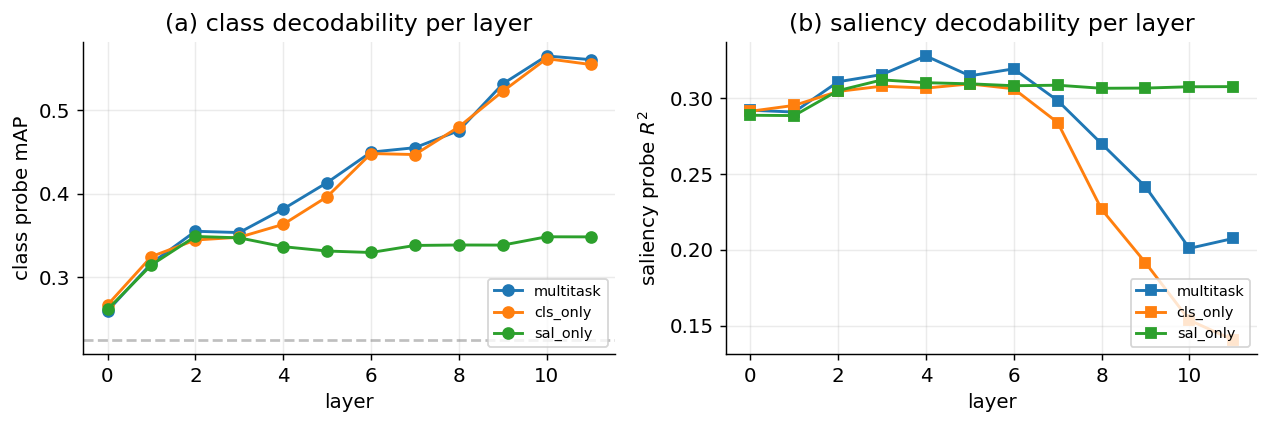
\includegraphics[width=0.92\linewidth]{probes_focused.png}
\end{center}
\vspace{-2pt}
\footnotesize
\textbf{Higher is better on both panels.} mAP $\in [0, 1]$ measures how well a linear probe can predict class labels from the layer's activations. $R^2 \in [-\infty, 1]$ measures how much of the saliency-map variance the probe explains.
\begin{itemize}\setlength\itemsep{1pt}
\item Class mAP at the final layer: \textcolor{mtblue}{multi-task $0.561$}, \textcolor{clsorange}{cls-only $0.555$}, \textcolor{salgreen}{sal-only $0.348$}.
\item Saliency $R^2$ at the final layer: \textcolor{salgreen}{sal-only $0.308$}, \textcolor{mtblue}{multi-task $0.208$}, \textcolor{clsorange}{cls-only $0.141$}.
\end{itemize}
Multi-task gets full classification decodability and partial saliency decodability.
\end{frame}

\begin{frame}{One-Slide Variant Summary}
\begin{center}
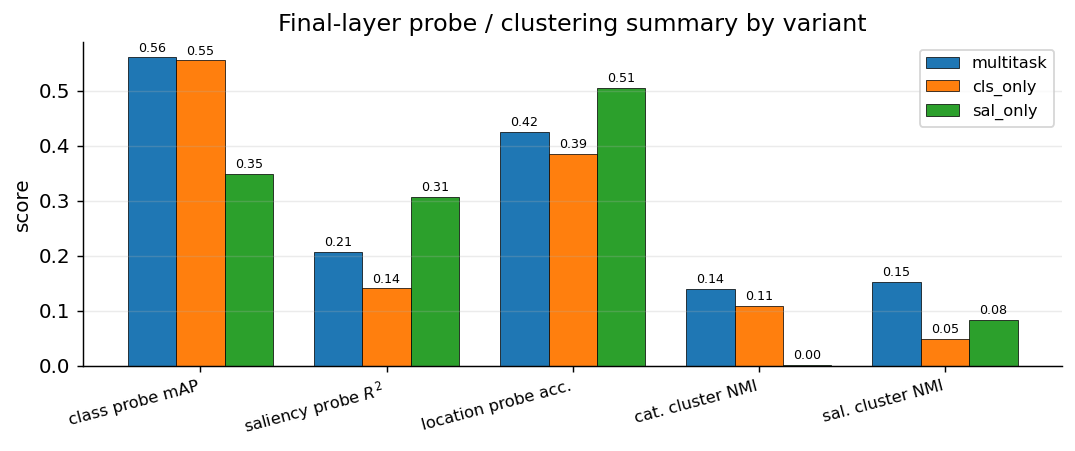
\includegraphics[width=0.92\linewidth]{variant_summary.png}
\end{center}
\vspace{-2pt}
\footnotesize
\textbf{Higher is better on every metric.} All five are scores in roughly $[0, 1]$, with $0$ meaning random and higher values meaning the layer encodes more of that signal. Across all five, the multi-task variant matches or beats both single-task variants on every axis except the one each was trained for. It is the only variant whose patch-token clusters carry both category and saliency structure (NMI $0.140$ and $0.153$).
\end{frame}

\begin{frame}{Pairwise Similarity, All 12 Layers}
\begin{center}
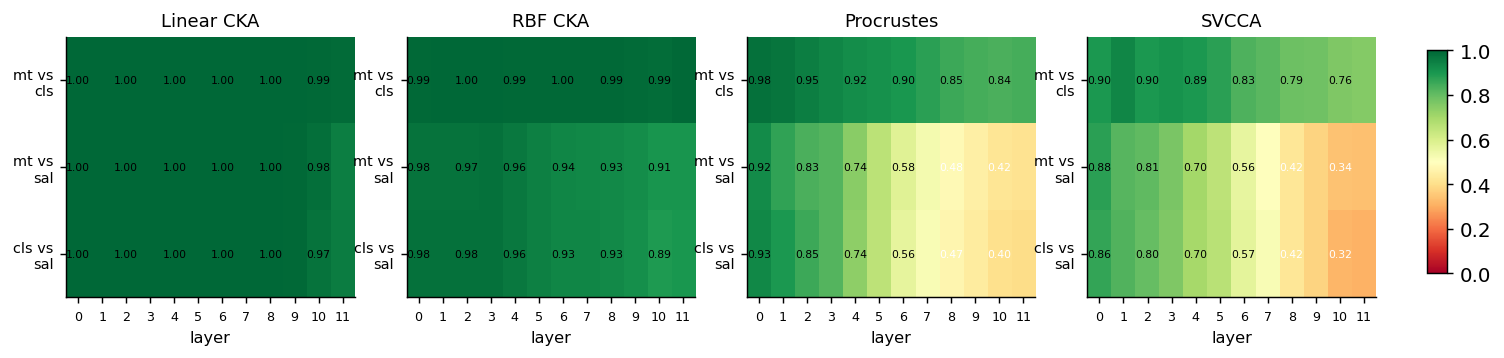
\includegraphics[width=\linewidth]{cka_heatmap.png}
\end{center}
\vspace{-2pt}
\footnotesize
\begin{itemize}\setlength\itemsep{1pt}
\item Linear and RBF CKA stay green throughout: every pair, every layer, $\geq 0.90$. CKA cannot tell the variants apart.
\item Procrustes and SVCCA reveal the asymmetry by mid-network. multi-task vs.\ cls-only stays warm-green. The two pairs involving sal-only fall into orange and red by layers 8 to 11.
\end{itemize}
\end{frame}

\begin{frame}{Final-Layer Similarity, Side by Side}
\begin{center}
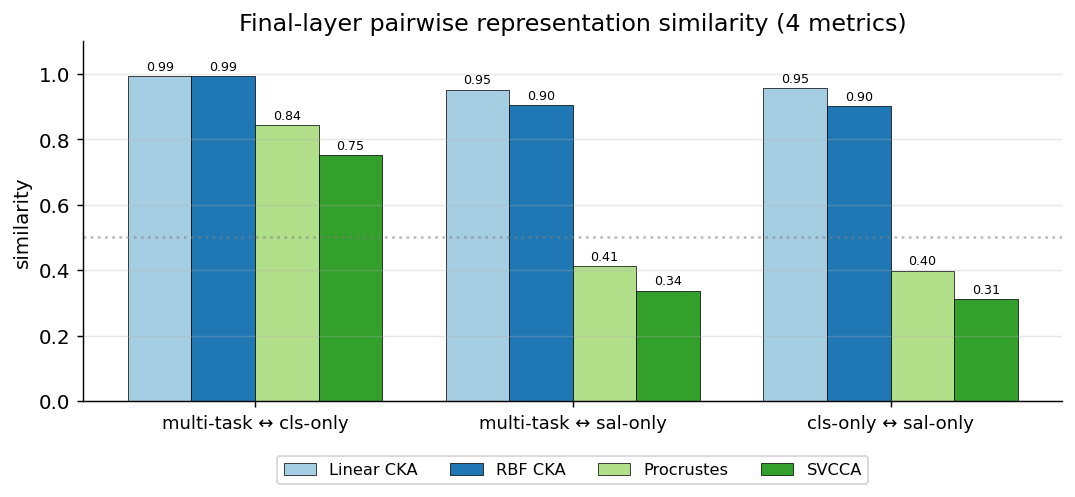
\includegraphics[width=0.85\linewidth]{final_layer_bars.png}
\end{center}
\vspace{-2pt}
\footnotesize
\textbf{Higher = more similar} (all four metrics are in $[0, 1]$, with $1$ meaning identical activations and $0$ meaning unrelated).
\begin{itemize}\setlength\itemsep{1pt}
\item multi-task vs.\ cls-only: Procrustes $0.84$, SVCCA $0.75$.
\item multi-task vs.\ sal-only: Procrustes $0.41$, SVCCA $0.34$.
\item cls-only vs.\ sal-only: Procrustes $0.40$, SVCCA $0.31$.
\end{itemize}
\textbf{The multi-task backbone's geometry inherits from cls-only, not sal-only.}
\end{frame}

\begin{frame}{Why CKA Was Insufficient}
\footnotesize
\textbf{The trap.} Linear CKA gave essentially no signal: every variant pair scored $\geq 0.95$ at every layer.
\vfill
\begin{itemize}\setlength\itemsep{2pt}
  \item Davari et al.\ (2023). CKA can be made arbitrarily high under subset-translation of the activation matrix. Saturation is documented.
  \item Cui et al.\ (2022). CKA is confounded by input-population structure, so even random networks can score high.
  \item Murphy et al.\ (2024). Even debiased CKA has limited resolution at low sample size.
\end{itemize}
\vfill
\textbf{Procrustes} (orthogonal alignment after centering and Frobenius normalization) and \textbf{SVCCA} (canonical correlation between top-$k$ singular subspaces) avoid both pitfalls and gave us the headline result.
\vfill
\textbf{Methodological recommendation.} When comparing models that share initialization or training regime, never rely on CKA alone.
\end{frame}

\begin{frame}{Patch-Token Clustering: Which Signal Each Variant Encodes}
\footnotesize
\resizebox{\linewidth}{!}{%
\begin{tabular}{lccccc}
\toprule
Variant & Cat.\ Purity & \textbf{Cat.\ NMI} & Sal.\ Purity & \textbf{Sal.\ NMI} & Stab.\ ARI \\
\midrule
\textcolor{mtblue}{Multi-task}      & $0.661$ & $\mathbf{0.140}$ & $\mathbf{0.558}$ & $\mathbf{0.153}$ & $0.606$ \\
\textcolor{clsorange}{Classifier-only} & $0.644$ & $0.109$ & $0.442$ & $0.049$          & $0.649$ \\
\textcolor{salgreen}{Saliency-only}  & $0.636$ & $0.001$ & $0.486$ & $0.084$          & $\mathbf{0.763}$ \\
\bottomrule
\end{tabular}}
\vspace{2pt}
\textbf{Metric definitions} (all in $[0, 1]$, higher is better):
\begin{itemize}\setlength\itemsep{0pt}
\item \textbf{Purity}: fraction of tokens whose cluster's plurality label matches the token's true label. Sensitive to cluster-size imbalance.
\item \textbf{NMI} (normalized mutual information): how much information cluster assignment shares with the true label, normalized so random clustering is $0$ and perfect agreement is $1$.
\item \textbf{ARI} (adjusted Rand index): chance-corrected agreement between two clusterings. We use it for seed-to-seed stability ($1$ = identical clusters across seeds, $0$ = chance).
\end{itemize}
\vspace{2pt}
\begin{itemize}\setlength\itemsep{0pt}
\item \textcolor{mtblue}{\textbf{Multi-task}} is the only variant whose clusters carry both category and saliency structure.
\item \textcolor{salgreen}{\textbf{sal-only}} clusters carry essentially no class signal (NMI $0.001$ is at the random floor).
\end{itemize}
\end{frame}

\begin{frame}{SAE Feature Ablation}
\begin{center}
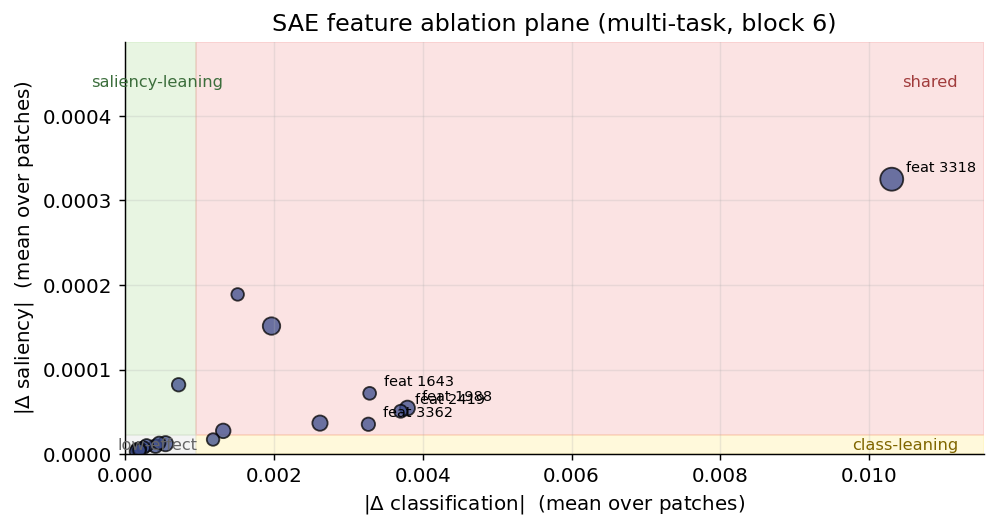
\includegraphics[width=0.6\linewidth]{sae_taxonomy.png}
\end{center}
\vspace{-3pt}
\scriptsize
An \textbf{SAE feature} is one of the 4096 sparse-dictionary directions the autoencoder learns. Each dot is one feature. We write $\Delta\text{cls}$ for the average change in the classification head's output when that feature is zeroed out, and $\Delta\text{sal}$ for the same change on the saliency head. Far right means class-driving. Far up means saliency-driving. Quadrants are split at the medians.
\begin{itemize}\setlength\itemsep{0pt}
\item Most features land class-leaning. Large $\Delta$ cls, tiny $\Delta$ sal.
\item Top feature 3318 (active in $38\%$ of patches): $\Delta$ cls $= 0.010$, $\Delta$ sal $= 0.0003$.
\item No purely saliency-leaning feature at this $k{=}32$ sparsity.
\item \textbf{Caveat.} TopK SAEs are seed-unstable (Paulo \& Belrose 2025). Exploratory.
\end{itemize}
\end{frame}

\begin{frame}{Attribution Baselines: Grad-CAM vs.\ Kernel SHAP}
\begin{center}
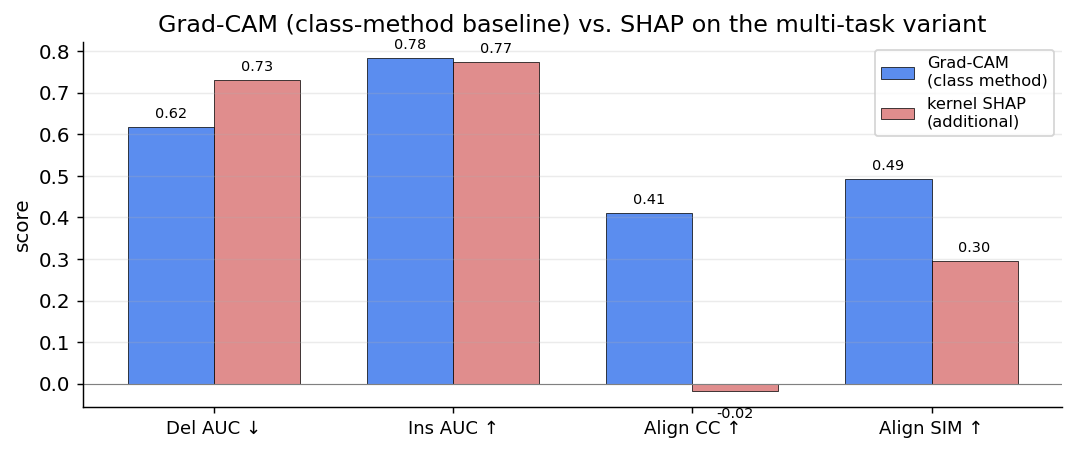
\includegraphics[width=0.85\linewidth]{attribution_bars.png}
\end{center}
\vspace{-2pt}
\footnotesize
\begin{itemize}\setlength\itemsep{1pt}
\item Grad-CAM CC $= 0.41$. This is the highest of any method across both projects (Project 1 best was IG at $0.25$).
\item Kernel SHAP CC $\approx 0$. No human alignment, even though Del and Ins AUC are comparable.
\item \textbf{Pattern.} Representation-space methods (Grad-CAM, IG) align with human gaze. Perturbation-based methods (LIME, SHAP) do not.
\end{itemize}
\end{frame}

% ============================================================
\section{Discussion}
% ============================================================

\begin{frame}{Putting the Story Together}
\footnotesize
\textbf{Going back to the central question.} Are Project 1's attribution-map differences anchored in real internal differences?
\vfill
\textbf{Answer: yes, and asymmetrically.}
\begin{enumerate}\setlength\itemsep{1pt}
  \item Multi-task and classifier-only are geometrically close in the second half of the network (Procrustes $0.84$, SVCCA $0.75$).
  \item Saliency-only is far from both (Procrustes $\approx 0.41$, SVCCA $\approx 0.33$).
  \item Multi-task's clusters are the only ones simultaneously aligned with COCO categories and saliency quartiles.
  \item SAE feature ablation: class effects roughly $10\times$ saliency effects on the same heads.
\end{enumerate}
\vfill
\textbf{Reading.} Multi-task supervision adds saliency-aligned structure on top of a still-dominantly-classifier-aligned representation. It does not reorganize the backbone from scratch.
\end{frame}

\begin{frame}{Limitations}
\footnotesize
\begin{itemize}\setlength\itemsep{3pt}
  \item \textbf{Single backbone, single dataset.} DeiT-Small and SALICON/COCO top-20 only. Larger ViTs and CNNs may behave differently.
  \item \textbf{SAE results are exploratory.} One layer (block 6), one seed, $4096$-feature dictionary. Paulo \& Belrose (2025) showed only $\sim 30\%$ of TopK features overlap across seeds, so any feature-inventory claim would need multi-seed work.
  \item \textbf{Kernel SHAP under sample budget.} 200 mask samples per image is below the standard for accurate Shapley estimates. Population CC $\approx 0$ is robust to this. Per-image attributions are noisy.
  \item \textbf{Probing $n{=}1000$ on 384-dim activations} is small relative to dimensionality. Probe results would benefit from $n \geq 10{,}000$.
\end{itemize}
\end{frame}

\begin{frame}{Future Work}
\footnotesize
\begin{itemize}\setlength\itemsep{3pt}
\item \textbf{Cross-variant SAEs with shared dictionary} (Lindsey et al.\ 2024 crosscoder style). Train one SAE on activations of all three variants jointly to formally identify shared, classifier-leaning, and saliency-leaning features.
\item \textbf{ERF-based feature interpretation} (Han, Kim, Kwak 2025) instead of activation-pattern interpretation, since attention mixing makes naive max-activating-patch readings misleading on ViTs.
\item \textbf{Replicate the asymmetry on a CNN backbone.} Tests whether multi-task-inherits-from-classifier is architecture-specific or general.
\item \textbf{Bigger probing $n$, more SAE seeds, factorial three-factor ablation} for a methodology-paper version.
\end{itemize}
\end{frame}

\begin{frame}{Five Takeaways}
\footnotesize
\begin{enumerate}\setlength\itemsep{2pt}
\item The multi-task ViT is asymmetrically classifier-aligned. It is closer to cls-only than to sal-only by mid-network.
\item Linear CKA was uninformative. Procrustes and SVCCA carried the analysis. Use multiple similarity metrics whenever variants share initialization.
\item Multi-task's patch-token clusters are the only ones simultaneously aligned with COCO categories and saliency quartiles.
\item SAE feature ablation: class effects roughly $10\times$ saliency effects (single-seed caveat applies).
\item Grad-CAM achieved CC $0.41$ against human saliency, the best alignment across both projects. Kernel SHAP achieved $\approx 0$, mirroring Project 1's LIME finding.
\end{enumerate}
\end{frame}

\begin{frame}
\begin{center}
\Large\textbf{Questions?}

\vfill
\normalsize
Nicholas Welsh \\
\texttt{nwelsh2024@my.fit.edu} \\
\vspace{0.5cm}
\href{https://github.com/nickvpn/vit-ml-xai-project}{github.com/nickvpn/vit-ml-xai-project}
\end{center}
\end{frame}

\end{document}
